\subsection{Two Important Kinds of ICs} 

%\DTMnewdatestyle{dateupdated}{〈definition 〉

Answers to M\Alph{subsection} problems are on page \pageref{opamps_digital_prob_answers}.  \textbf{\textcolor{red}{Updated \DTMnow.}}

%--------------------------------------------------------------------------------------------------------------
\begin{Exercise}
\label{prob_calculate_inverting_amp_gain}
For the circuit shown below, suppose that $V_{\rm in} =3$~volts.  
Find (a)~$V_+$ and $V_-$, 
(b)~$I_{R3}$ and $I_{R4}$, 
(c)~$\Delta V_{R3}$ and $\Delta V_{R4}$.  
(d)~What direction does current flow in $R_3$ and in $R_4$: to the left or to the right? 
(e)~Which direction does current flow through the op-amp's output? 
(f)~What is $V_{\rm out}$?

\vspace{-0.15in}
\begin{center}
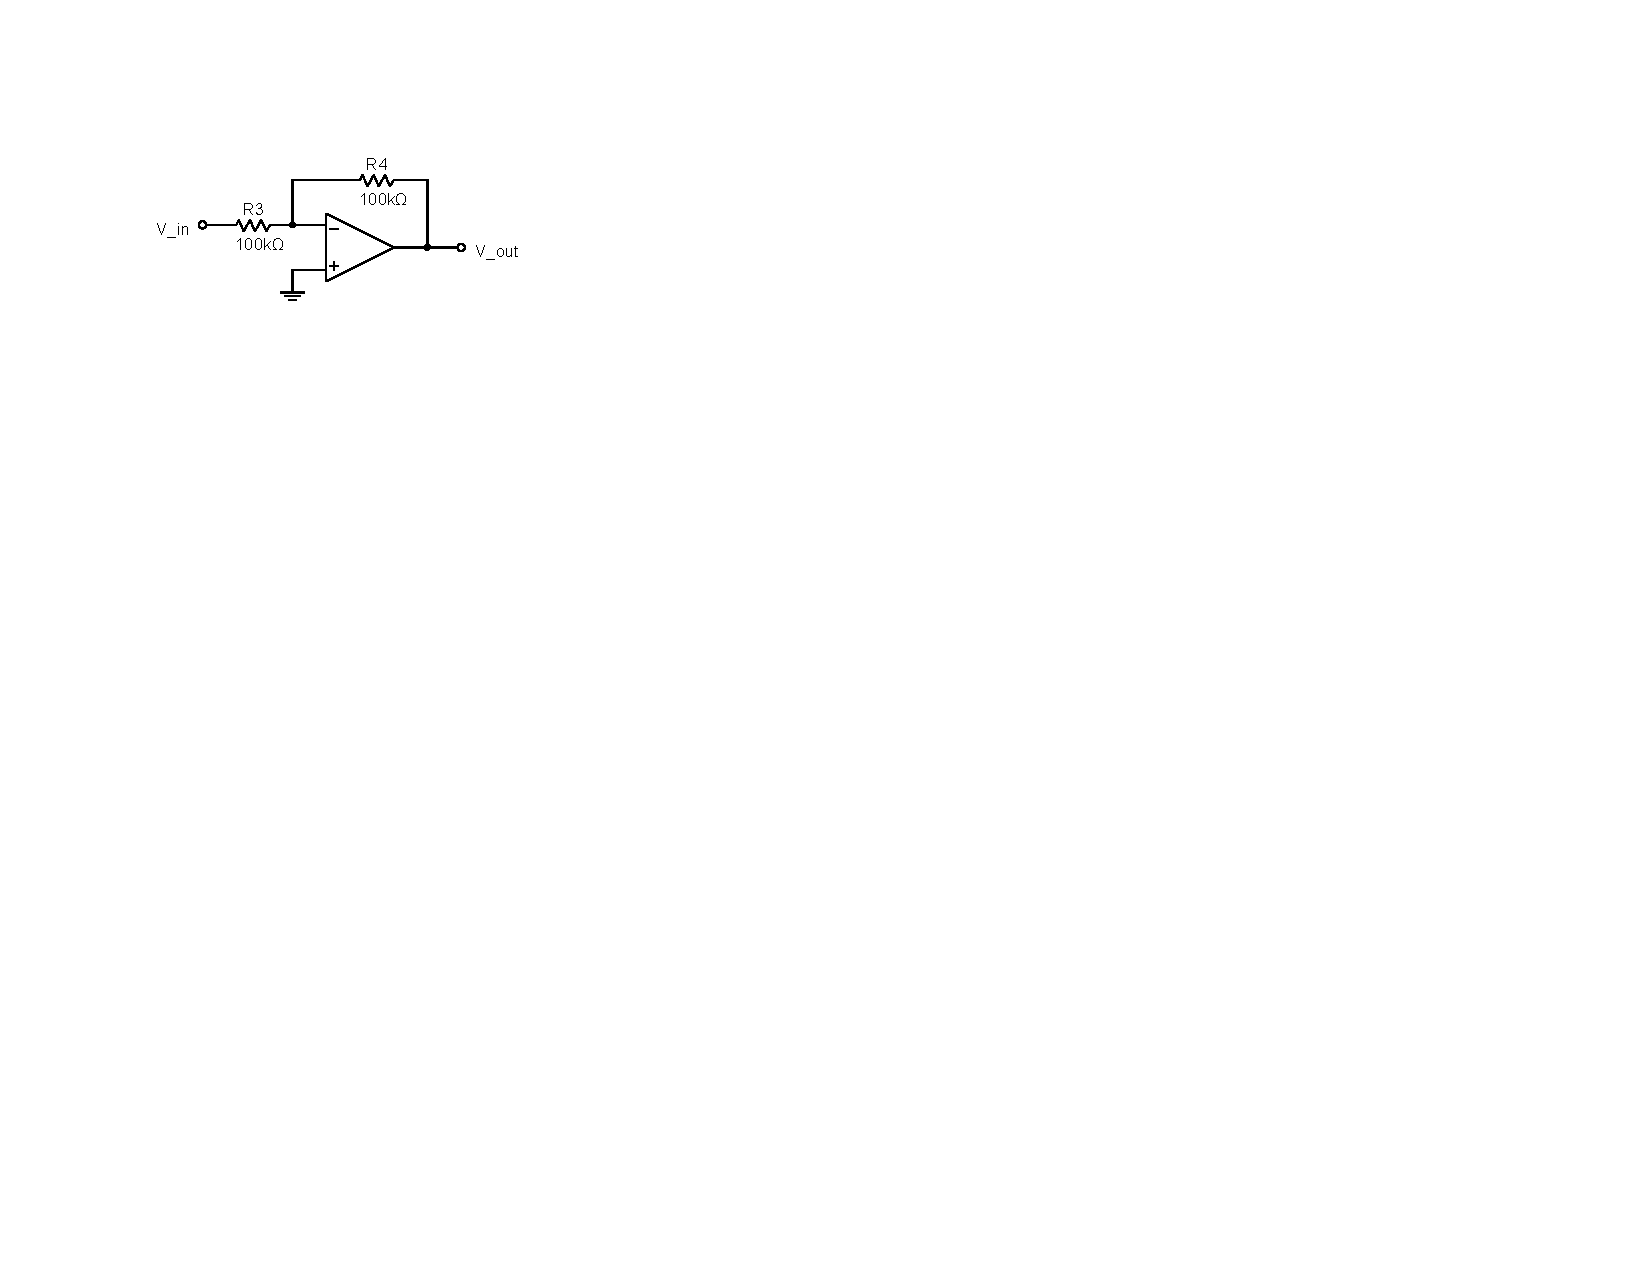
\includegraphics{M_problems/opamps_digital/inverting.pdf}
\end{center}
\vspace*{-0.25in}
\end{Exercise}
\begin{Answer}
(a) 0 (b) $30~\mu$A (c) 3 volts (d) both flow left to right (e) right to left (f) $-3$ volts
\end{Answer}

%--------------------------------------------------------------------------------------------------------------
\begin{Exercise}
\label{prob_thevenin_equiv_for_2V_supply}
A student named Ralph has used a voltage divider to build a 2-volt DC voltage supply, shown below on the left.  It turns out there is a very useful theorem by a fellow named Thevenin, which says roughly the following:
\begin{quote}
``Any collection of voltage sources and resistors (even the crazy middle figure below!) is functionally equivalent to a single voltage source $V_{\rm Th}$ and a single internal resistance $R_{\rm Th}$ as shown on the right.  No measurement at $V_{\rm out}$ can distinguish between the two circuits.''  ---L\'eon Charles Th\'evenin (heavily paraphrased).
\end{quote}
In this problem, you will calculate the values of $V_{\rm Th}$ and $R_{\rm Th}$ for the equivalent circuit of Ralph's voltage supply. 

\vspace{-0.15in}
\begin{center}
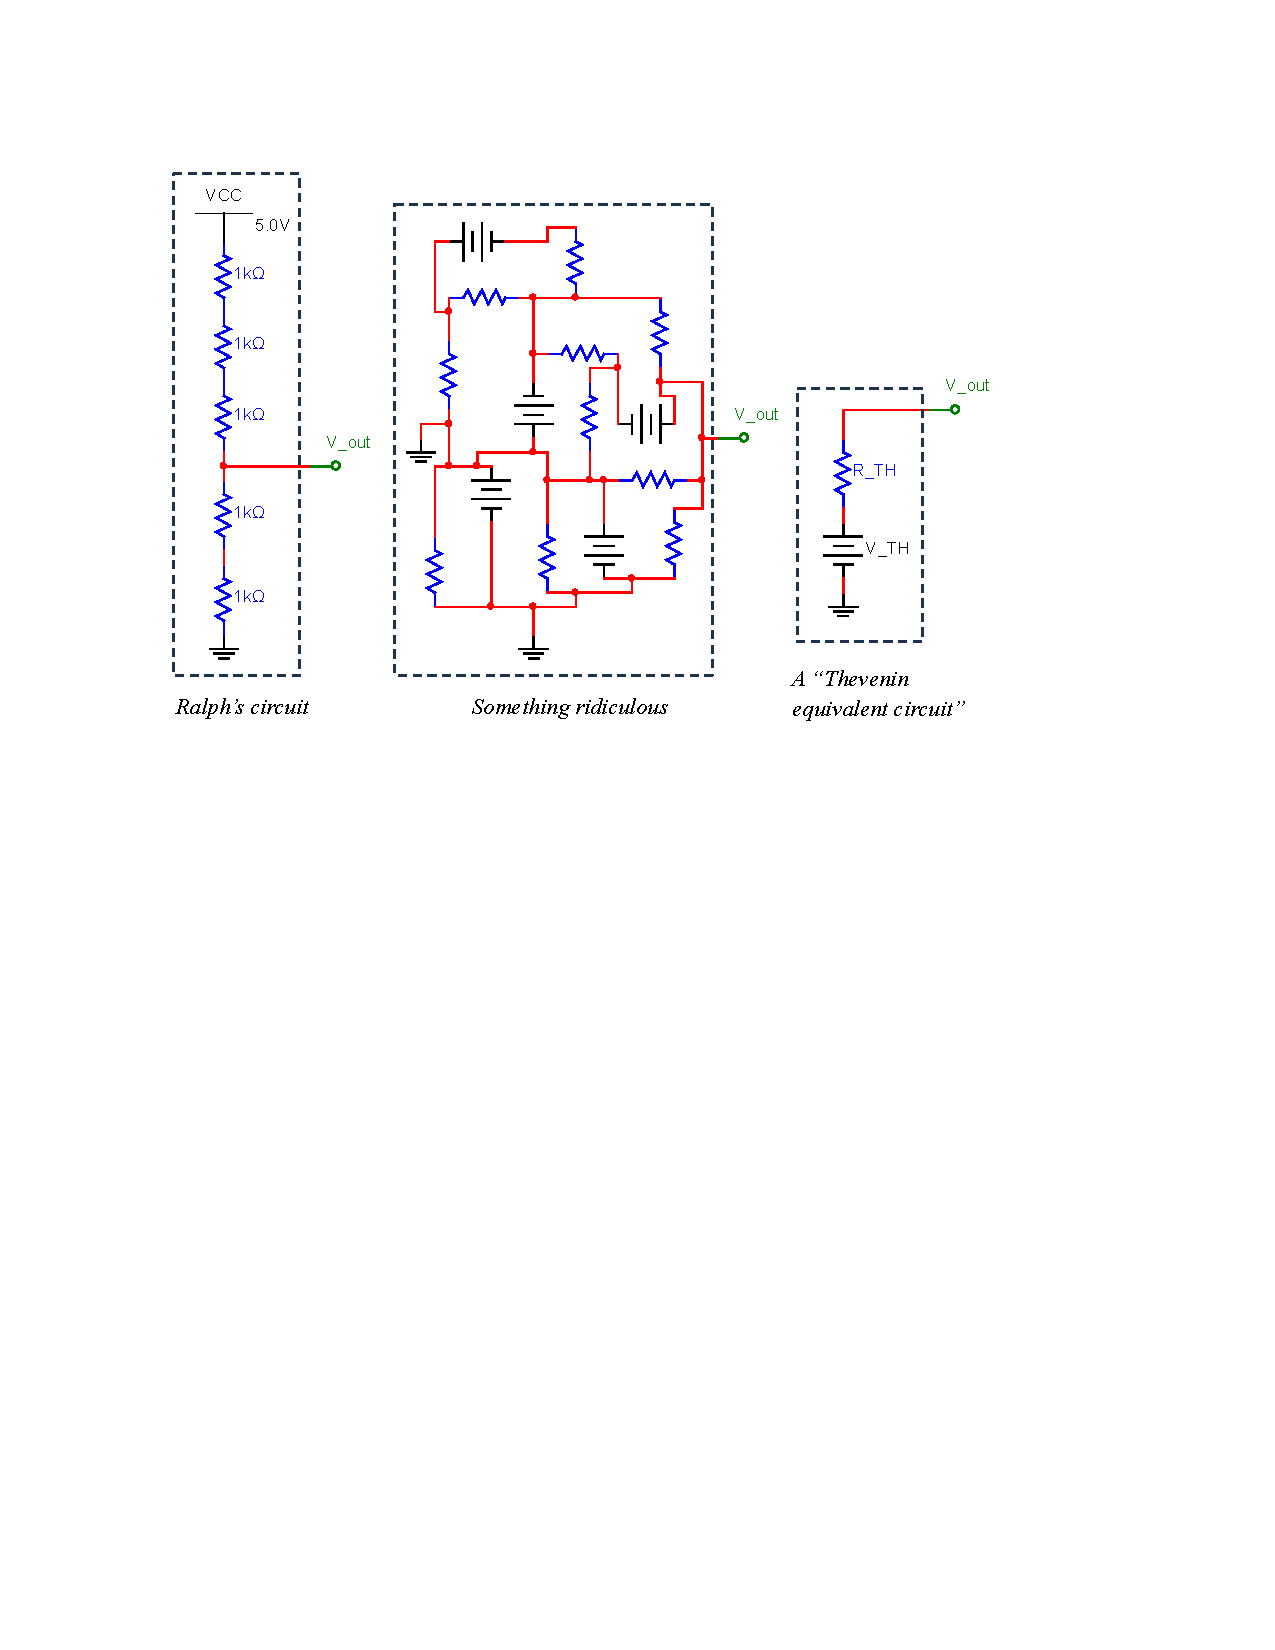
\includegraphics[scale=0.86]{M_problems/opamps_digital/thevenin_equivalence.pdf}
\index{color page}
\end{center}
\vspace{-0.25in}

\begin{enumerate}[label=(\alph*),nosep]
\item What is the open-circuit voltage of the Thevenin equivalent circuit on the right, in terms of $V_{\rm Th}$ and $R_{\rm Th}$? 
\item What is the short-circuit current of the Thevenin equivalent circuit on the right? 
\item What is the open-circuit voltage of Ralph's circuit?  
\item What is the short-circuit current of Ralph's circuit?  
\item From your previous parts what are the values of $V_{\rm Th}$ and $R_{\rm Th}$ for Ralph's circuit?  
\item Ralph does the same calculation that you did, and says, ``Hey, it looks like the output impedance of my circuit is 1.2~k$\Omega$.''  Is \textit{output impedance} the right thing for Ralph to call it?
\end{enumerate}
For more help using Thevenin's theorem, see Appendix \ref{thevenin_equivalence}.
\end{Exercise}
\begin{Answer}
(a) It's just $V_{\rm Th}$ (b) $V_{\rm Th}$ and $R_{\rm Th}$ (c) 2 V (d) 1.67 mA (e) 2 V and 1.2 k$\Omega$ (f)~Sure, that's basically what it is.  In this context, ``output impedance/resistance'' or ``internal resistance'' or ``Thevenin equivalent resistance'' basically all mean the same thing.
\end{Answer}


%--------------------------------------------------------------------------------------------------------------
\begin{Exercise}
In this problem, you will test whether Ralph's circuit in the previous problem is equivalent to a Thevenin equivalent circuit with $V_{\rm Th}=2$~volts and $R_{\rm Th}=1.2\kohm$, by checking the behavior of a circuit with a single, arbitrarily chosen load resistor $R_{\rm L}$. Suppose a load  $R_{\rm L}=2.7\kohm$ is connected between Ralph's output and ground.  (a)~Calculate the voltage across and current through $R_{\rm L}$ by analyzing the circuit in the diagram below on the left.  (b)~Calculate the voltage and current for $R_{\rm L}$ by analyzing the circuit in the diagram below on the right.  (c)~Are they the same?  (d)~Does this count as a ``proof'' of Thevenin's theorem?
\begin{center}
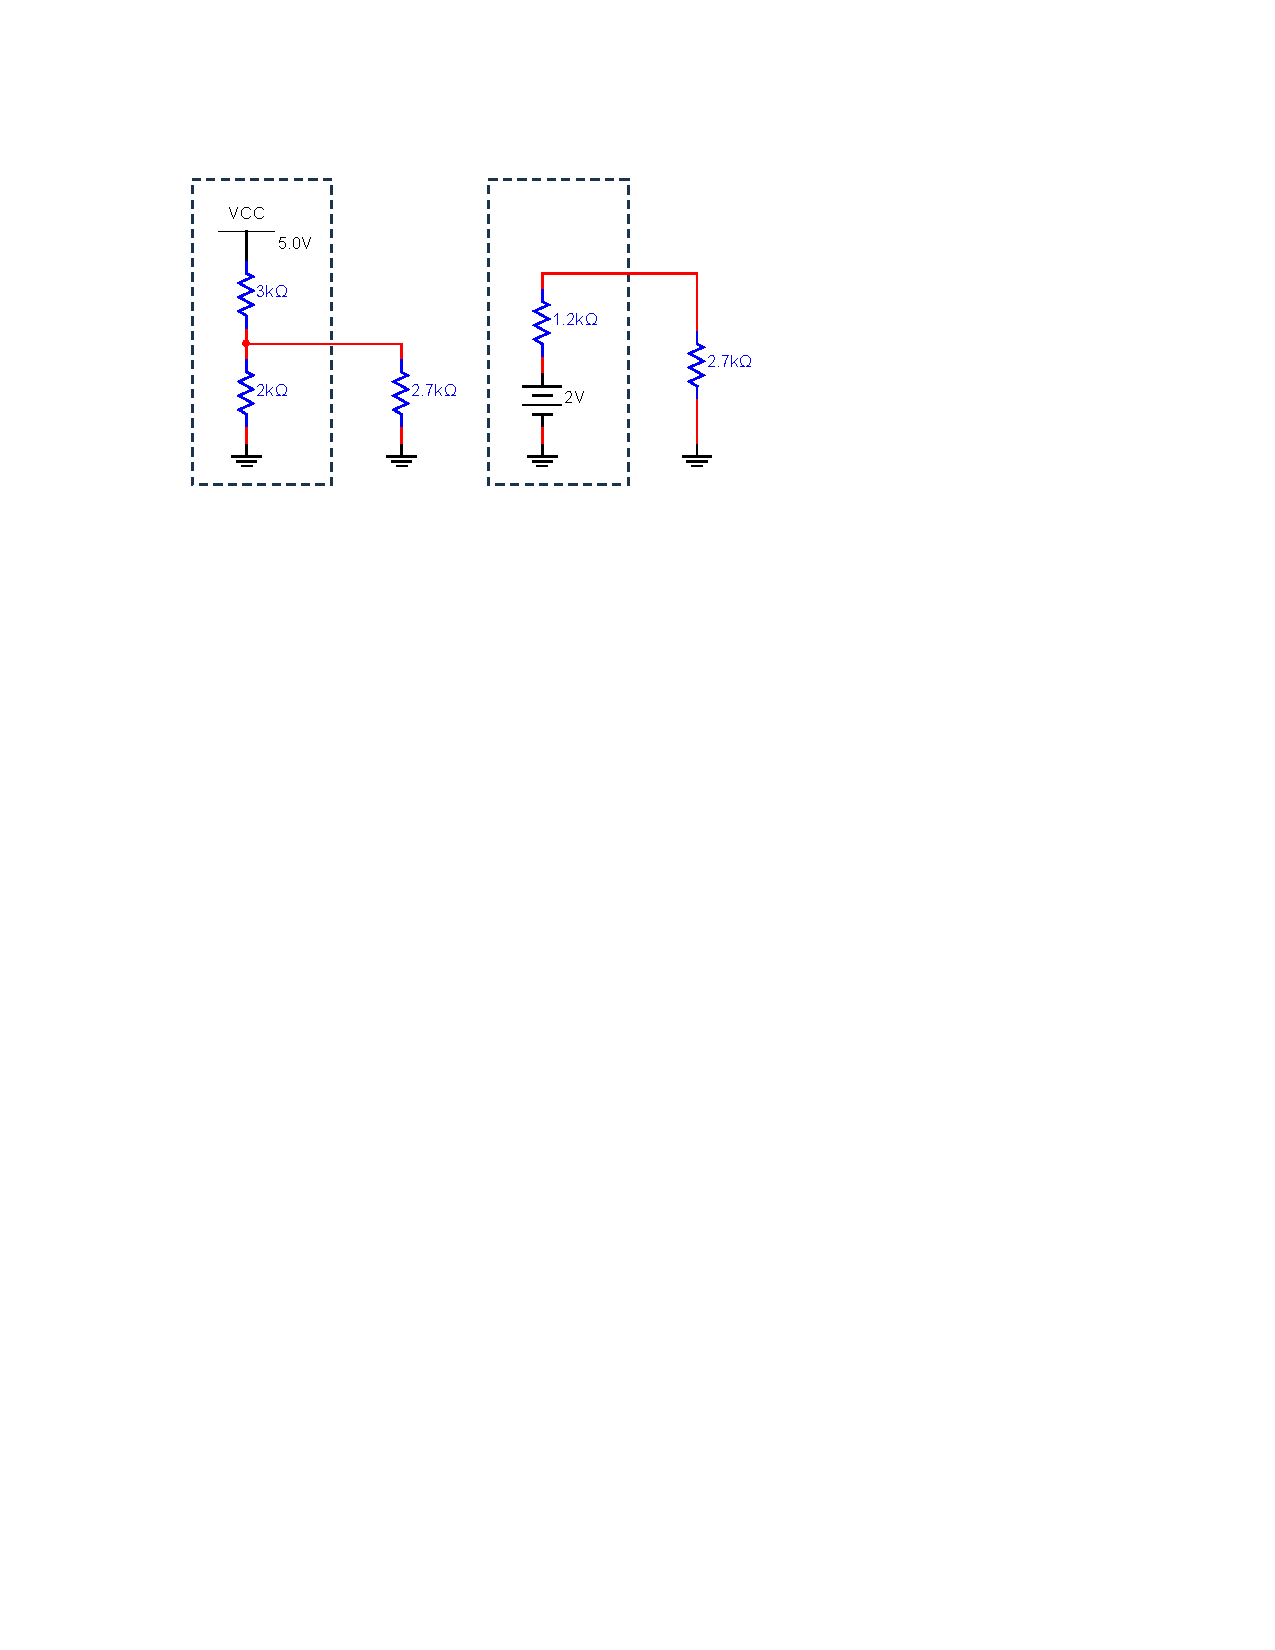
\includegraphics[scale=0.9]{M_problems/opamps_digital/thevenin_equivalence2.pdf}
\index{color page}
\end{center}
\end{Exercise}
\begin{Answer}
(a)~1.38~V and 513~$\mu$A  (c)~They'd better both be the same! (d)~No, it's not a general proof, because you demonstrated it only for one specific load (a single $2.7\kohm$ resistor) connected to one specific circuit made by some fake guy named Ralph.  But if you see this kind of thing enough times, it does start to seem convincing.  :-)
\end{Answer}


%--------------------------------------------------------------------------------------------------------------
\begin{Exercise}
\label{prob_amplifier_input_impedances}
(a) What is the input impedance of the inverting amplifier you built in Lab \ref{lab_op-amps}, part \ref{part_inverting_amplifier}?  
(b) By contrast, is the input impedance of the non-inverting amplifier you built in Lab \ref{lab_op-amps} part \ref{part_non-inverting_amplifier} larger or smaller than the inverting amplifier?
(c) What additional information would you need in order to calculate a numerical value for the input impedance of the non-inverting amplifier, and where would you go to find it?
\end{Exercise}
\begin{Answer}
(a) Hint: The input $V_+$ is at ground, and the op-amp adjusts its output to keep $V_- = V_+$.  This means that the $V_-$ input is essentially at 0 volts as well---what we call a \textit{pseudo ground}---and you can treat it as if the right side of resistor $R_3$ was simply connected directly to ground.
\end{Answer}

%--------------------------------------------------------------------------------------------------------------
\begin{Exercise}
Anna and Bob are building inverting amplifiers, just as you did in Lab \ref{lab_op-amps}, part \ref{part_inverting_amplifier}. Their goal is to use a 2-volt signal as an input to an inverting amplifier with a gain of $-1$.  Anna builds the circuit on the left (below), and Bob builds the circuit in the middle. 
(a)~Which of the two circuits works the way it's supposed to, and why does the other one \textit{not} work?
(b)~Carla is out of $100\kohm$ resistors, so she builds the circuit on the right.  Show how to calculate the output voltage of Carla's circuit \textit{specifically by using the results from problems
\textsl{\ref{prob_thevenin_equiv_for_2V_supply}} and
\textsl{\ref{prob_amplifier_input_impedances}}.}
\begin{center}
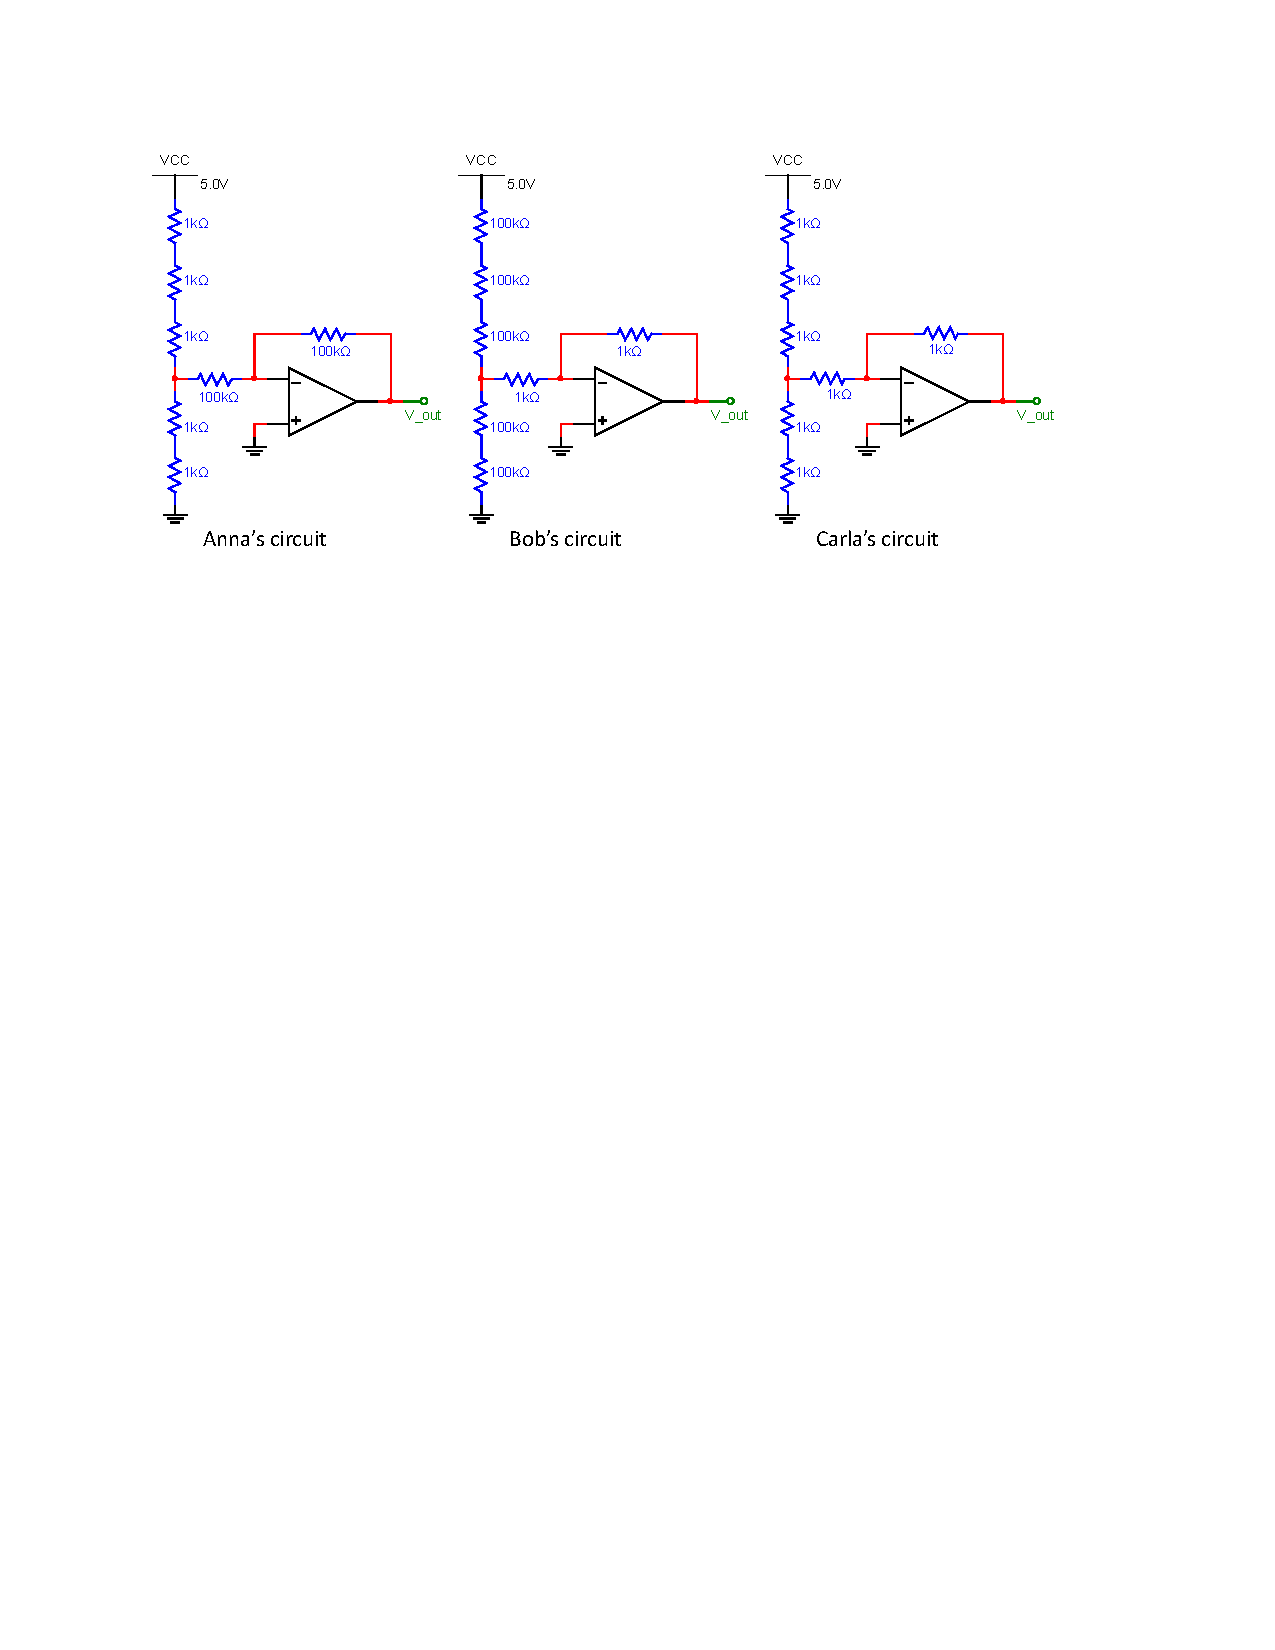
\includegraphics{M_problems/opamps_digital/anna_bob_carla.pdf}
\end{center}
\end{Exercise}
\begin{Answer}
(b) $-0.91$~volts
\end{Answer}


%--------------------------------------------------------------------------------------------------------------
\begin{Exercise}
Referring to the circuit diagrams in parts 
\ref{part_non-inverting_amplifier} and 
\ref{part_inverting_amplifier} of 
Lab \ref{lab_op-amps}, 
\textit{derive} (using a judicious mix of math, words, and/or pictures)  expressions for (a)~the gain $G$ of a non-inverting amplifier in terms of $R_1$ and $R_2$, and (b)~the gain $G$ of an inverting amplifier in terms of $R_3$ and $R_4$.
\end{Exercise}
\begin{Answer}
(a) $G=\left(R_1 + R_2\right) / {R_2}$ (b) $G={-R_4}/{R_3}$.  General hint: In problem \ref{prob_calculate_inverting_amp_gain} you worked out the gain of an inverting amplifier with specific resistor values, and you can follow the same kind of logic here.
\end{Answer}


%--------------------------------------------------------------------------------------------------------------
\begin{Exercise}
A source with an output impedance of 50 ohms produces an open-circuit sinusoidal voltage with an amplitude of 300~mV.  The source is connected to an audio amplifier with voltage gain $G=200$, input impedance $R_{\rm in} = 600\ohm$, and output impedance $R_{\rm out} = 2\ohm$.  The output of the amplifier is connected to a speaker with an impedance of $4\ohm$.  (You don't need to worry about the inner workings of the amplifier other than that it produces an internal source emf $\varepsilon$ that is 100 times larger than the voltage across its internal $600\ohm$ resistance; that is, $\varepsilon = 100 \times V_{\rm input}$.
(a) Find the amplitude of the voltage across the speaker. 
(b) Suppose the audio amplifier has a maximum current output of 30~A.  What is the maximum amplitude of the input voltage to the amplifier, above which the sinusoidal output to the speaker would be ``clipped'' as you saw in 
Lab \ref{lab_op-amps}
part \ref{part_clipping}?
\begin{center}
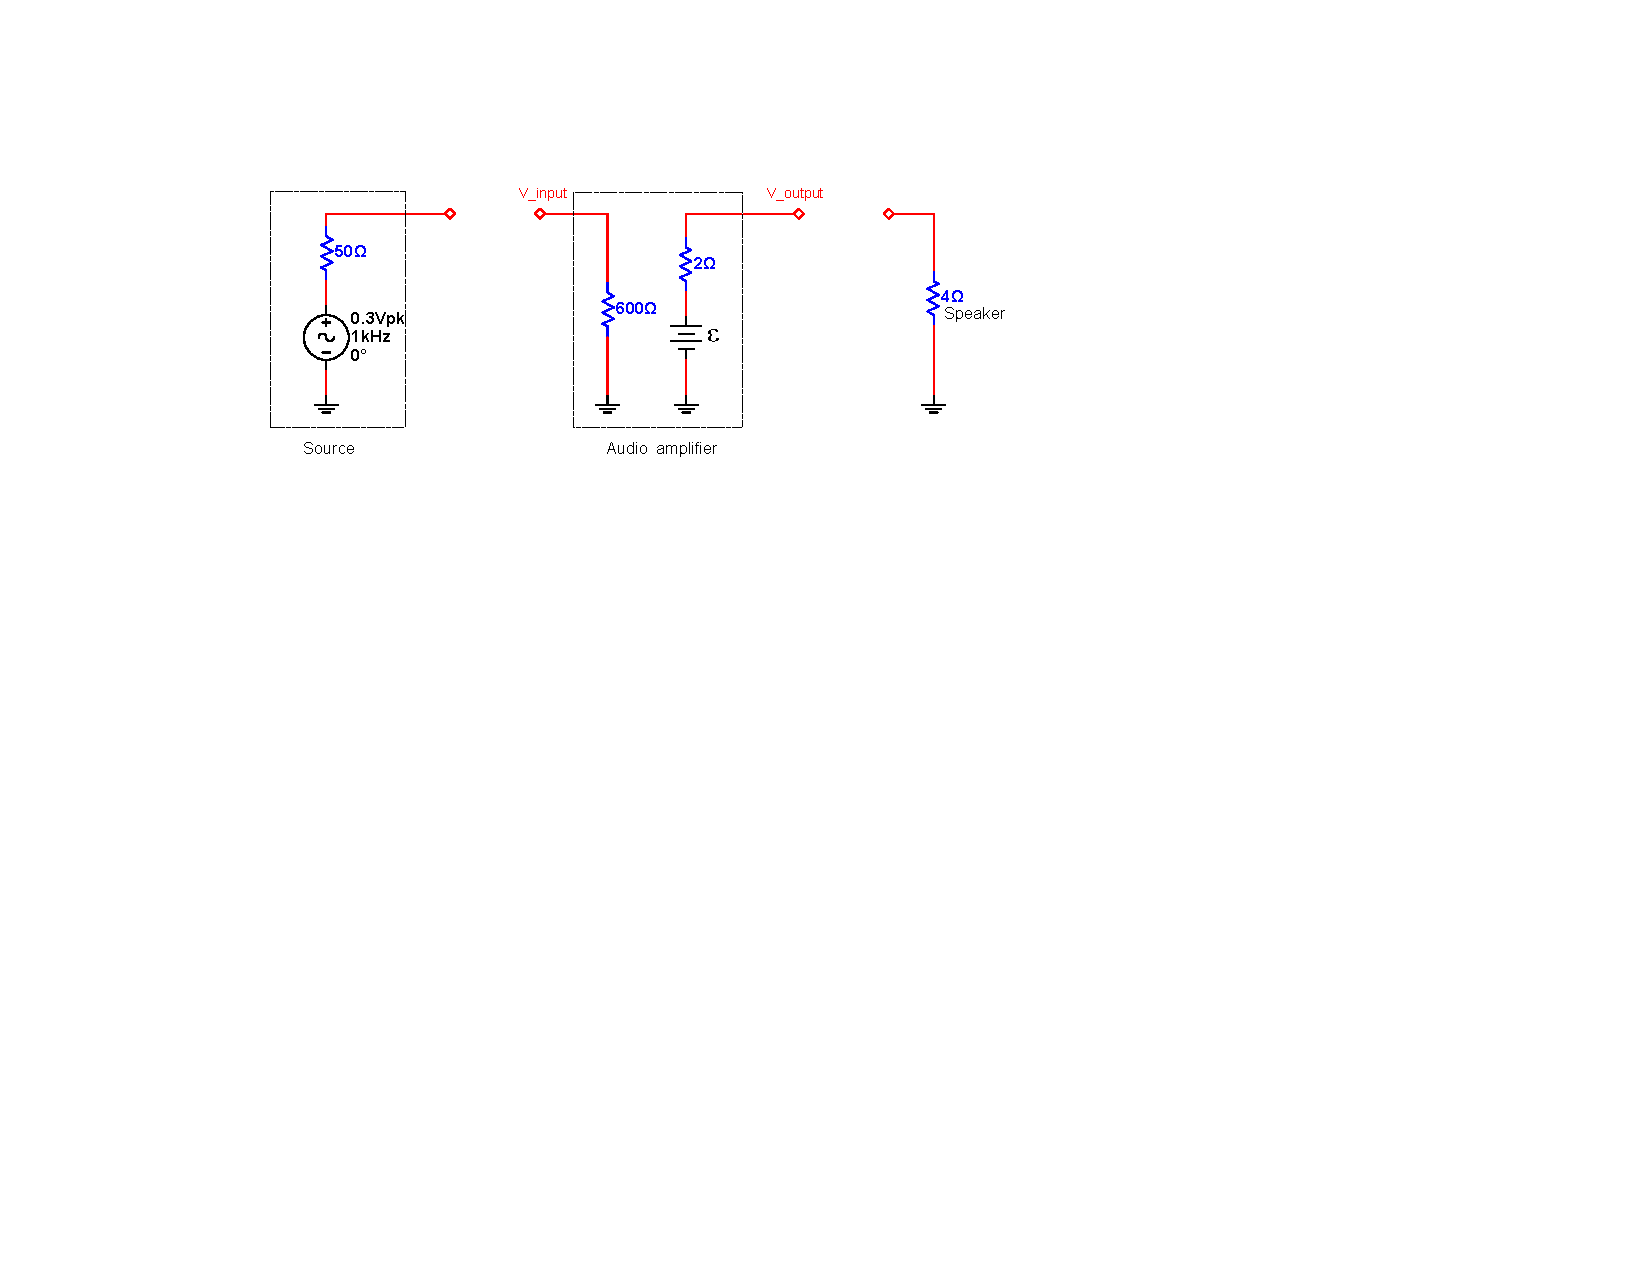
\includegraphics{M_problems/opamps_digital/audio_amplifier.pdf}
\end{center}
\end{Exercise}
\begin{Answer}
(a) 37 V (b) 900 mV
\end{Answer}

%--------------------------------------------------------------------------------------------------------------
\begin{Exercise}
Goofus and Gallant have been learning about op-amps.  Goofus believes that by flipping the $V_+$ and $V_-$ terminals of the op-amp, he has invented a handy way to build a non-inverting summing amplifier, shown below:
\begin{center}
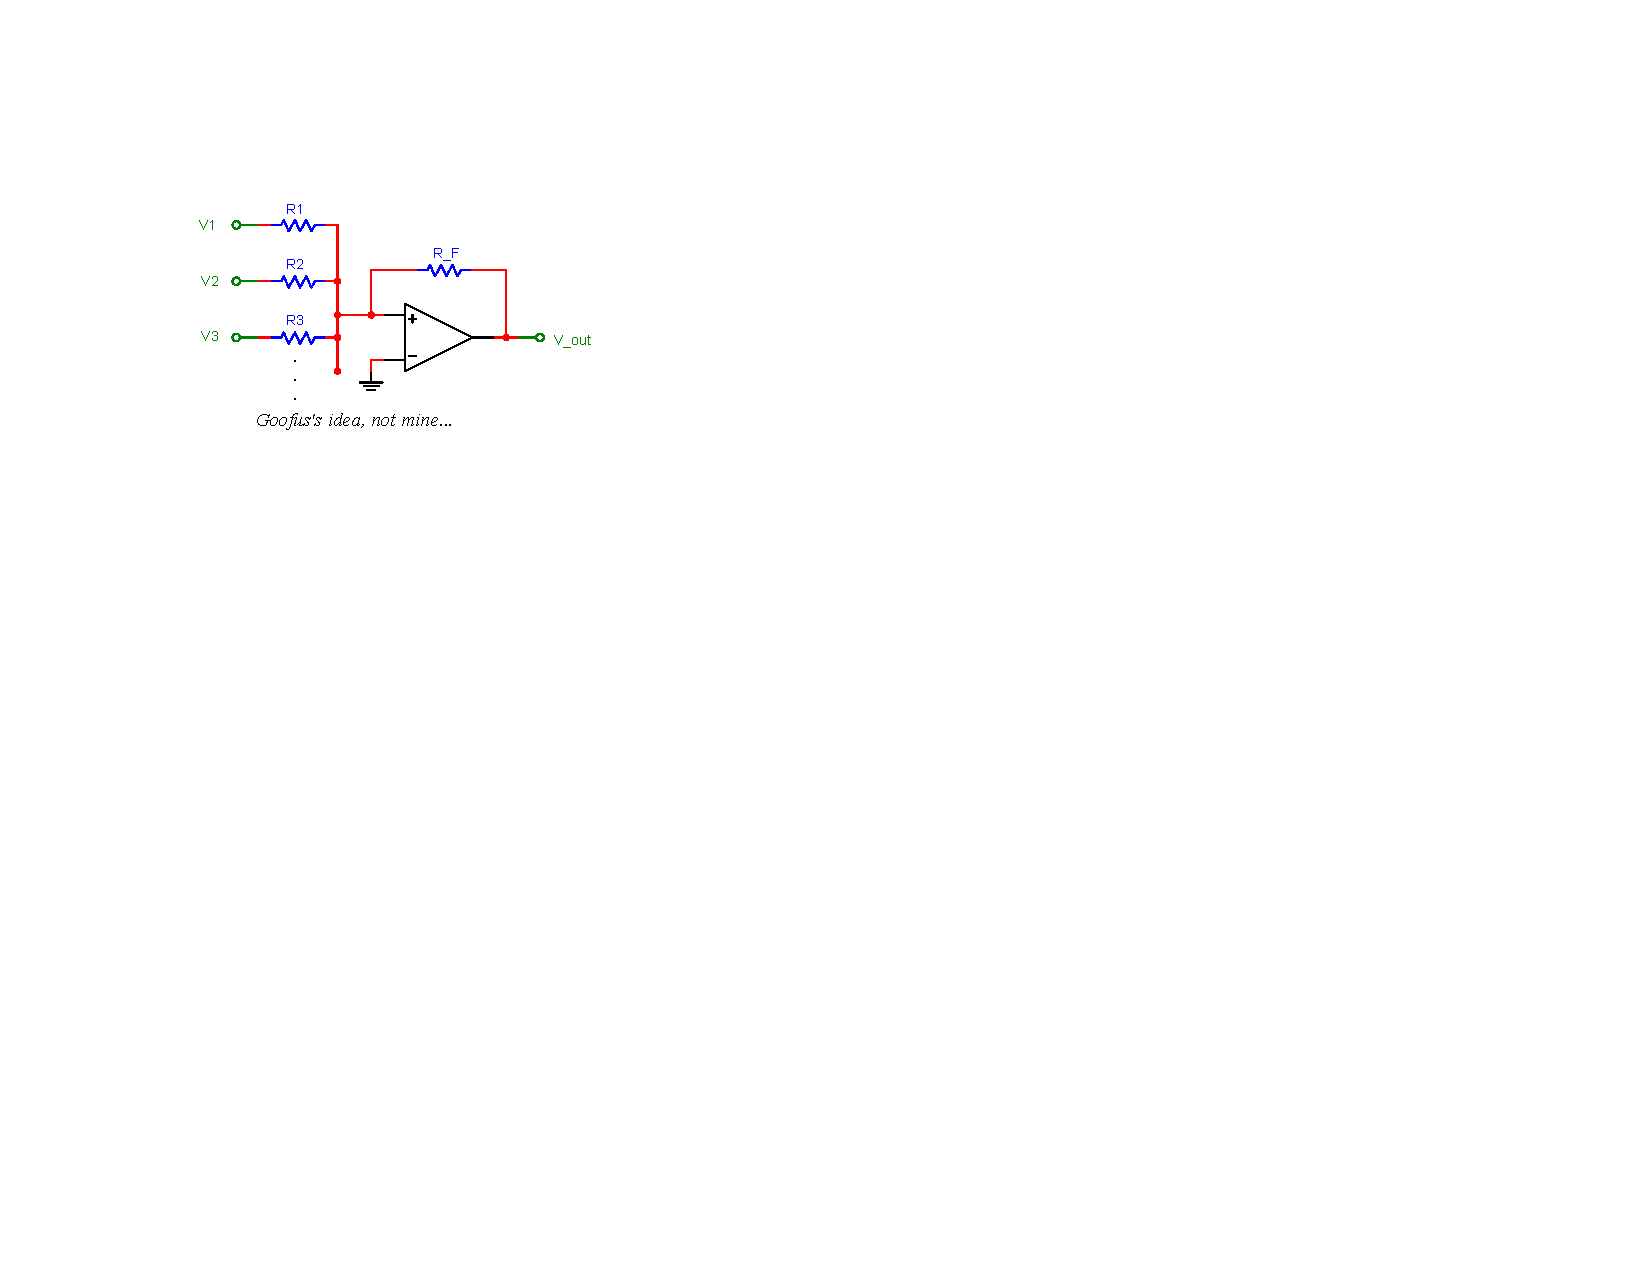
\includegraphics{M_problems/opamps_digital/summing_amp_goofus.pdf}
\end{center}
Goofus explains to Gallant that it should work perfectly, according to the golden rules:
\begin{itemize}[nosep]
\item By Golden Rule 2, $V_+=V_-=0$ volts.
\item By Golden Rule 1, no current flows into the $V_+$ input, so 
$I_{RF}=\dfrac{V_1}{R_1} +  \dfrac{V_2}{R_2}+\dfrac{V_3}{R_3} .$
\item Based on the current through $R_F$, the output should be 
$V_{\rm out}=+R_F \left( \dfrac{V_1}{R_1} +  \dfrac{V_2}{R_2}+\dfrac{V_3}{R_3} \right)$.
\end{itemize}
\vspace{-0.1in}
\begin{enumerate}[label=(\alph*),nosep]
\item Write a short, condescending email from Gallant to Goofus that explains what's wrong with his reasoning.  
\item Include in your email what the output of his circuit would \textit{actually} be were he to build it, \textit{and why}.
\end{enumerate}
\end{Exercise}
\begin{Answer}
Hints:
(a)~Your explanation to Goofus will almost surely involve the words \textit{feedback, negative,} and \textit{positive}.
(b)~The actual output is guaranteed to be either $\approx+15$~V or $\approx-15$~V, pinned at one of the two power rails.  But Goofus won't intuit this on his own, so you still need to explain to him why.
\end{Answer}


%--------------------------------------------------------------------------------------------------------------
\begin{Exercise}
A noninverting amplifier with a gain $G=5$ (as in 
Lab \ref{lab_op-amps} 
part \ref{part_inverting_amplifier}) 
needs to provide an output of 30~mA to a load at $V_{\rm out}=5$~volts.  (That is, the load resistance is $R_{\rm load}=167\ohm$.) 
The maximum output current of the op-amp is 40~mA. 
(a)~What are the minimum values of the two resistors $R_1$ and $R_2$ that could be used, so that they don't draw too much current?  
(b) Why might very large values for the two resistors, like in the range of several $\Mohm$ or more, also cause your circuit to not work correctly? Note: to avoid these two problems, your default should be to pick $R_1$ and $R_2$ (the ``feedback resistors'') in the $10\kohm$ or $100\kohm$ ranges.  If you do that, you don't have to worry about it or calculate anything; it'll mostly just work.
\end{Exercise}
\begin{Answer}
(a) $100\ohm$ and $400\ohm$ (b) Hint: what might be a realistic value for the input impedance of the $V_-$ input?
\end{Answer}

%--------------------------------------------------------------------------------------------------------------
\begin{Exercise}
The circuit below is essentially a differential amplifier, but with unusual values of all four resistors.  It's not obvious what the use of such a circuit would be, but set that aside and use the ``golden rules'' of op-amps to calculate 
(a)~the voltages at the inputs $V_+$ and $V_-$, 
(b)~the output voltage $V_{\rm out}$, and 
(c)~the output current of the op-amp.  (That is, the current coming out of the output pin of the op-amp, not necessarily the current in the load resistor.)  
\begin{center}
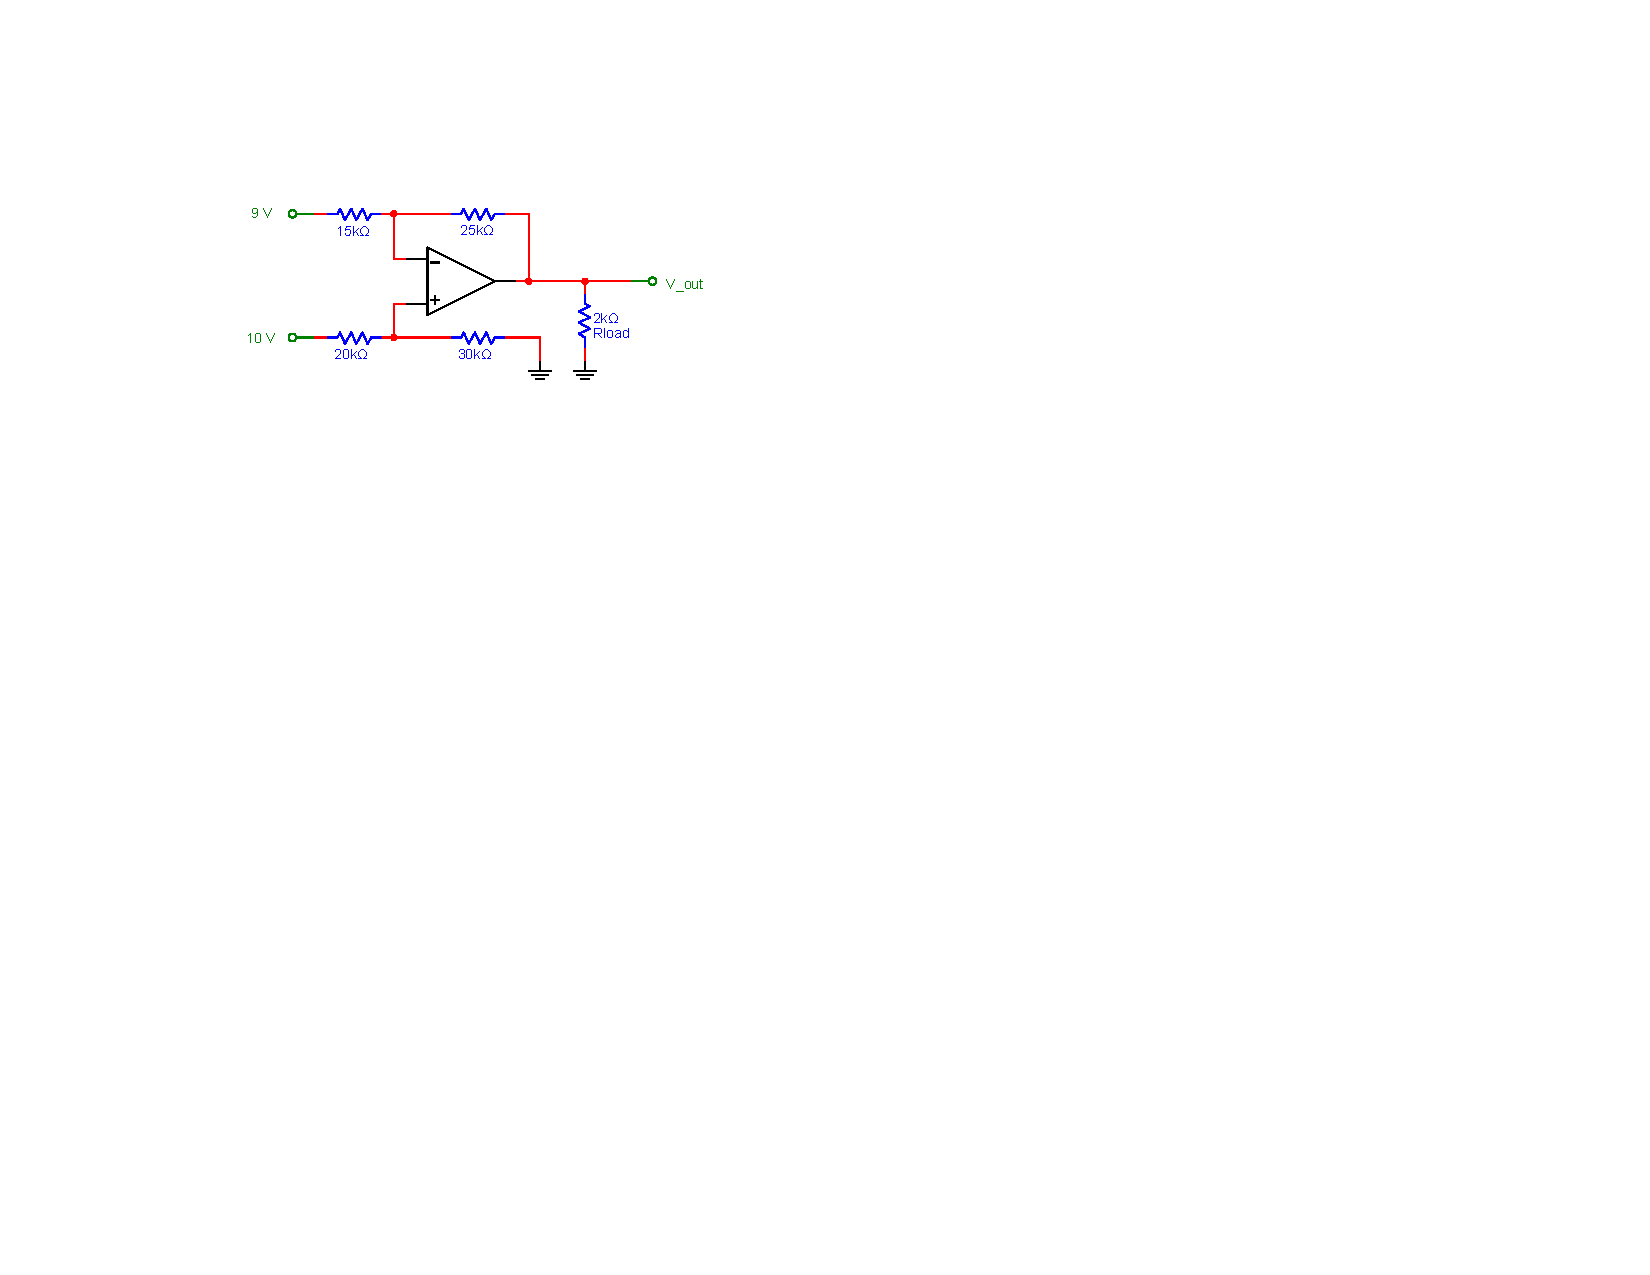
\includegraphics{M_problems/opamps_digital/differential_amp_odd.pdf}
\end{center}
\end{Exercise}
\begin{Answer}
(a)  $V_+=V_-=6$ volts  (b) 1 volt (c) 300 $\mu$A
\end{Answer}

%--------------------------------------------------------------------------------------------------------------
\begin{Exercise}
On page 749 of our textbook by Paynter, the author relates an op-amp's maximum usable frequency to its slew rate by plunking down Equation 22.5,
$$f_{\rm max}=\frac{{\rm slew~rate}}{2\pi V_{\rm pk}},$$
with no explanation of where it might come from or why it might be true.  Derive this equation, providing the explanation that Paynter left out.  Incidentally, the lack of motivation for equations like this is one of the reasons I'm not crazy about this book.  I suspect it stems in part from the assumption that the readers' math ability is so exceptionally low that they are just \textit{barely} able to plug numbers into a formula that's provided for them, laboriously pressing the calculator buttons with their knuckle pads and then requiring a long rest. 
\end{Exercise}


%Ideas for additional problems:

\vspace{0.75in plus 0.75in minus 0.2in} 

%\pagebreak[3]
\textbf{Answers to Selected {\thesubsection} Problems:}
\label{opamps_digital_prob_answers}
%\shipoutExercise
\shipoutAnswer

\cleardoublepage
